\section{A Distributed Solution Framework with Partial Information}
% Algorithm with Partial Information
\label{sec:algorithm}
%TODO: algorithm with a name
In this section, we shall introduce a novel approximation method to decouple the centralized optimization on the RHS of the Bellman's equations in equation (\ref{eqn:sp_0}) to each AP for arbitrary system state.
For the APs outside the conflict AP sets of each other, the update of dispatching actions at one AP will not affect the task computation originated from other APs.
Thus, the optimization of their dispatching actions can be decoupled.
On the other hand, for the APs within the same conflict AP set, the optimization of their dispatching actions is coupled.
Due to the unknown signaling latency, it is difficult for one AP (say the $k$-th AP) to predict the update of the dispatching actions at the other APs ($\forall k' \in\ccSet_{k}$).
Hence, cooperative optimization of dispatching actions for the APs within the same conflict AP set is infeasible.
In this section, we introduce an \emph{alternative policy iteration algorithm}, called \algname, to optimize the dispatching actions of one AP in a conflict AP set in each broadcast interval periodically, while other APs maintain their dispatching actions in the previous broadcast interval.
Specifically, the proposed distributed algorithm consists of the following two steps:
%\hongyc{(move two steps adjacent in the following subsections)}
\begin{enumerate}
    \item We first introduce a baseline policy, use its value function to approximate the value function of the optimal policy $\Policy^*$, and derive the analytical expression of the approximate value function for arbitrary GSI in Section \ref{subsec:baseline}.
    \item With the approximate value function, in Section \ref{subsec:ap_alg}, \hongyc{the AP set is partitioned into multiple independent subsets with a heuristic greedy algorithm and the \algname~is proposed,}
    %an alternative action update algorithm
    where only a subset of APs are selected to update their dispatching actions distributedly in each broadcast interval.
    Moreover, the analytical performance bound is also derived in Section \ref{subsec:analysis}.
\end{enumerate}
As a remark notice that solving the value function and then the RHS of the Bellman's equations are the two standard steps to solve an MDP problem with complete knowledge on system state.
In our proposed approximate solution framework, we extend this procedure to the POMDP problem in P1 by exploiting the structure of partially connected edge computing systems.
To the best knowledge of authors, a POMDP can hardly be solved via the Bellman's equations of full system state knowledge in the existing literature.

\subsection{Baseline Policy and Approximate Value Function}
\label{subsec:baseline}
To alleviate the curse of dimensionality, we first use the baseline policy $\Baseline$ with fixed dispatching actions to approximate value function at the RHS of the Bellman's equations in equation (\ref{eqn:val_f}).
Specifically, the baseline policy is elaborated below.
% Specifically, the baseline policy we used in this paper is elaborated below.

\begin{definition}[Baseline Policy]
    In the baseline policy $\Baseline$, each AP fixes the target processing edge server for each job type as the previous broadcast interval. Specifically, at the $t$-th broadcast interval,
    {\small
    \begin{align}
        \Baseline\Paren{\Stat(t),\Delay(t)} &\define \Brace{ 
            \Pi_{1}(\Stat_{1}(t),\mathcal{D}_{1}(t)),
            \dots,
            \Pi_{K}(\Stat_{K}(t),\mathcal{D}_{K}(t))
        },
    \end{align}
    }
    where
    \begin{align}
        \Pi_{k}\Paren{\Stat_{k}(t),\mathcal{D}_{k}(t)}
        &= \Brace{
            {\omega}_{k,j}(t+1) \Big| \forall j\in\jSpace
        }, \forall k\in\apSet.
    \end{align}
\end{definition}

\hongyc{Specifically, the initial dispatching actions ($\omega_{k,j}(0), \forall j\in\jSpace$) of the $k$-th AP adopt the values as follows.}
\begin{align}
    \omega_{k,j}(0) = \arg\min_{m} u_{k,m,j} \vec{R}^{(k)}_{m,j}(0, 0) 
    \\
    + c_{m,j} (Q_{m,j}(0,0) + \|\|\vec{R}^{(k)}_{m,j}(0, 0)\|\| + 1)
\end{align}

\begin{example}[Time-related Fixed Actions in Baseline Policy]
    \hongyc{
        (Give an example why baseline policy is time-related;
        if the baseline policy not updated at $t=0$, it would be ...;
        if the baseline policy only updated once, it would be ...)
    }
\end{example}

Let $W_{\Baseline}(\cdot)$ be the value function of the baseline policy $\Baseline$, we shall approximate the value function of the optimal policy $V(\cdot)$ via $W_{\Baseline}$, i.e.,
{\small
\begin{align}
    &V\Paren{\Stat(t+1)} \approx W_{\Baseline}\Paren{\Stat(t+1)}
    \nonumber\\
    =& \sum_{m\in\esSet,j\in\jSpace}\Brace{
        \sum_{k\in\apSet} \tilde{W}^{\AP}_{k,m,j}(\Stat(t+1))
        +\tilde{W}^{\ES}_{m,j}(\Stat(t+1))
    },
    \label{eqn:baseline}
\end{align}
}where $\tilde{W}^{\AP}_{k,m,j}(\Stat(t+1))$ denotes the cost raised by the type-$j$ jobs which are being transmitted from the $k$-th AP to the $m$-th edge server with the baseline policy $\Baseline$ and initial system state $\Stat(t+1)$, and $\tilde{W}^{\ES}_{m,j}(\Stat(t+1))$ denotes the cost raised by the type-$j$ jobs on the $m$-th server.
Their definitions are given below.
{\small
\begin{align}
    \tilde{W}^{\AP}_{k,m,j} \Paren{\Stat(t+1)} &\define
        \sum_{i=0}^{\infty} \gamma^{i+1} \mathbb{E}^{\Baseline}\Bracket{
            \Inorm{\vec{R}^{(k)}_{m,j}(t+i+1)}
        },
    \\    
    \tilde{W}^{\ES}_{m,j} \Paren{\Stat(t+1)} &\define
        \sum_{i=0}^{\infty} \gamma^{i+1} \mathbb{E}^{\Baseline}\Bracket{
            Q_{m,j}(t+i+1) +
            \nonumber\\
            &~~~~~~~~~~\beta I[Q_{m,j}(t+i+1) = L_{max}]
        }.
\end{align}
}

Moreover, the explicit expressions of $\tilde{W}^{\AP}_{k,m,j}(\Stat(t+1))$ and $\tilde{W}^{\ES}_{m,j}(\Stat(t+1))$ are derived in the following lemmas, respectively.

\begin{lemma}[Analytical Expression of $\tilde{W}^{\AP}_{k,m,j}$]
    \label{lemma:w_ap}
    \begin{align}
        &\tilde{W}^{\AP}_{k,m,j}\Paren{\Stat(t+1)} =
        \bigg\|
            \vecG{\Theta}^{(k, \Baseline)}_{m,j}(t+1) \times
            \Bracket{
                \mat{I} - \gamma \Gamma^{(k)}_{m,j}
            }^{-1}
        \bigg\|,
        \label{w_ap}
    \end{align}
    where $\mat{I}$ is the identity matrix, and $\vecG{\Theta}^{(k, \Baseline)}_{m,j}(t)$ and $\Gamma^{(k)}_{m,j}$ are defined below.
    \begin{itemize}
        \item {\small $\vecG{\Theta}^{(k,\Baseline)}_{m,j}(t) \define \Bracket{
            \theta^{(k,\Baseline)}_{m,j}(0,t),
            \theta^{(k,\Baseline)}_{m,j}(1,t),
            \dots,
            \theta^{(k,\Baseline)}_{m,j}(\Xi,t)
            }$},
        where 
        \begin{align}
            \theta^{(k,\Baseline)}_{m,j}(\xi,t) \define 
            \begin{cases}
                \lambda_{k,j} I[\omega_{k,j}(t)=m], & \xi=0
                \\
                \Pr\{R^{(k)}_{m,j}(\xi,t,0) = 1\}, & \text{otherwise}
            \end{cases}
        \end{align}
        denotes the probability that there is one type-$j$ job have been delivered from $k$-th AP to $m$-th edge server for $\xi$ time slots at the very beginning of the $t$-th broadcast interval, when the baseline policy $\Baseline$ is adopted;
        \item $\Gamma^{(k)}_{m,j} \in \mathbb{R}^{(\Xi+1)\times(\Xi+1)}$ denotes the transition matrix of $\vecG{\Theta}^{(k,\Baseline)}_{m,j}(t)$ ($\forall t$) under baseline policy $\Baseline$ whose entries are provided in Appendix \ref{append_1}.
    \end{itemize}
\end{lemma}
\begin{proof}
    Please refer to Appendix \ref{append_1}.
\end{proof}

\begin{lemma}[Analytical Expression of $\tilde{W}^{\ES}_{m,j}$]
    \label{lemma:w_es}
    {\small
    \begin{align}
        &\tilde{W}^{\ES}_{m,j}\Paren{\Stat(t+1)}
    = \sum_{i=0,\dots,\frac{\Xi}{T}} \gamma^{i} \mathbb{E}^{\Baseline}[ Q_{m,j}({t+i+1}) | \Stat(t+i)]
    \nonumber\\
    &~~~~~~~~~~~~+ \gamma^{\frac{\Xi}{T}} 
    \vecG{\nu}_{m,j}({t+\frac{\Xi}{T}+1})
    \Paren{
        \mat{I} - \gamma \mat{P}^{\Baseline}_{m,j}(t+\frac{\Xi}{T}+1)
    }^{-1} \vec{g}',
        \label{w_es}
    \end{align}   
    }
    where $\vecG{\nu}_{m,j}(t)$, $\mat{P}_{m,j}(\beta_{m,j}(t))$, $\beta_{m,j}(t)$ and $\vec{g}$ are defined below.
    \begin{itemize}
        \item {\small
        $\vecG{\nu}_{m,j}(t) \define [\Pr\{Q_{m,j}(t)=0\}, \dots, \Pr\{Q_{m,j}(t)=L_{max}\}]$
        } denotes the PMF (probability mass function) vector of $Q_{m,j}(t)$.
        \item $\vec{g} \in \mathbb{R}^{(L_{max}+1) \times 1}$ denotes the cost vector of edge server, and its $i$-th entry is
        \begin{align}
            [\vec{g}]_{i} \define 
            \begin{cases}
                i, & i=0,1,\dots,L_{max}-1
                \\
                L_{max}+\beta, & \text{otherwise}
            \end{cases}.
            \label{eqn:g_vec}
        \end{align}
        \item The expression of $\mathbb{E}^{\Baseline}[ Q_{m,j}({t+i+1}) | \Stat(t+i)]$ is elaborated in Appendix \ref{append_2}.
        \item $\mat{P}^{\Baseline}_{m,j}(t) \in \mathbb{R}^{(L_{max}+1) \times (L_{max}+1)}$ denotes the transition matrix of $\vecG{\nu}_{m,j}(t)$ under baseline policy $\Baseline$ whose entries are described in Appendix \ref{append_2}.
    \end{itemize}   
\end{lemma}
\begin{proof}
    Please refer to Appendix \ref{append_2}.
\end{proof}

\subsection{Distributed Action Update}
\label{subsec:ap_alg}
Although the optimal value function has been approximated via the baseline policy in the previous part, it is still infeasible for all the APs to solve the RHS of the Bellman's equations in a distributed manner with OSI and local \brlatency~only.
This is because the evaluation of equation (\ref{w_ap}) and (\ref{w_es}) requires the knowledge of GSI and \brlatency~at all APs.
Instead, it is feasible for part of APs to update their dispatching actions distributedly in each broadcast interval and achieve a better performance compared with baseline policy.
Hence, we first define the following sequence of AP subsets, where each subset are selected to update dispatching actions periodically.
\begin{definition}[Subsets Partition]
    Let $\mathcal{Y}_{1}, \dots, \mathcal{Y}_{N} \subseteq \apSet$ be a collection of subsets of AP set $\apSet$, which satisfy
    \begin{align}
        &\bigcup_{n=0,\dots,N-1} \mathcal{Y}_{n} = \apSet
        \label{eqn:subset_cup}
        \\
        \esSet_{y} \cap \esSet_{y'} &=\emptyset, y' \neq y~(\forall y',y \in \mathcal{Y}_{n}).
        \label{eqn:subset_disjoint}
    \end{align}
\end{definition}
The condition in equation (\ref{eqn:subset_cup}) is to ensure all the APs can update their dispatching actions periodically; whereas the condition in equation (\ref{eqn:subset_disjoint}) is to ensure APs in the conflict AP sets of each other will not update their dispatching actions in the same broadcast interval.
For example, as illustrated in Fig.\ref{fig:system}, the AP set $\apSet$ could be decomposed of two subsets as $\set{1,3}$ and $\set{2}$.
The subset partition is not trivial and a partition minimizing the update period $N$ is preferred.
A heuristic greedy algorithm is given in Algorithm \ref{alg_0}.
\begin{algorithm}[ht]
    \caption{Greedy Subset Partition Algorithm}\label{alg_0}
    \DontPrintSemicolon % Some LaTeX compilers require you to use \dontprintsemicolon instead
    \KwIn{$\apSet, \set{\esSet_{k}, \forall k\in\apSet}$ }
    \KwOut{a subset partition $\set{ \mathcal{Y}_{n} }$}
    Initialize a subset partition as $\mathcal{Y}_{n} = \set{n}$ ($\forall n\in\apSet$).\;
    \While{ $\exists \mathcal{Y}_a$ and $\mathcal{Y}_b$ ($a \neq b$), $\cup\set{ \esSet_{y}|y\in\mathcal{Y}_a } \bigcap \cup\set{ \esSet_{y}|y\in\mathcal{Y}_b } \neq \emptyset$ }
    {
        Count number of subsets in the current subset partition which have disjoint candidate set with $\mathcal{Y}_n$ ($\forall n$), denoted the number as $I_{n}$.\;
        $\tilde{n} \gets \arg\min_{n} I_{n}$\;
        Merge the subset $Y_{\tilde{n}}$ with one of its disjoint subsets.\;
    }
\end{algorithm}

At the $t$-th broadcast interval, the APs in the subset indexed with $n \define t \pmod{N}$ update their dispatching actions, while the other APs keep the same dispatching actions as the previous broadcast interval.
Hence, let
\begin{align}
    \tilde{\mathcal{A}}(t) \define \Brace{ {\omega}_{y,j}(t+1) \Big| \forall y\in\mathcal{Y}_{n},j\in\jSpace }
\end{align}
be the aggregation of dispatching actions of the APs in the subset $\mathcal{Y}_{n}$, and
\begin{align}
    \hat{\mathcal{A}}(t) \define \Brace{ {\omega}_{y,j}(t+1) \Big| \forall y\notin\mathcal{Y}_{n}, j\in\jSpace}
\end{align}
be the aggregation of dispatching actions of the rest APs, which are the same as the previous broadcast interval.
At the $t$-th broadcast interval, the optimization of $\tilde{\mathcal{A}}(t)$ at the RHS of the Bellman's equations can be rewritten as the following problem.
{\small
\begin{align}
    \textbf{P2:}~
    \min_{ \tilde{\mathcal{A}}(t) }
    &\sum_{\Stat(t+1)} \Pr\Brace{
        \Stat(t+1) \Big| \Stat(t), \hat{\mathcal{A}}(t), \tilde{\mathcal{A}}(t)
    } \cdot W_{\Baseline}\Paren{\Stat(t+1)}.
\end{align}
}

Moreover, we have the following conclusion on the decomposition of P2.
\begin{lemma}[]
    The optimization problem in P2 can be equivalently decoupled into local optimization problems at APs {for each subset partition}.
    Specifically, {the local optimization for each AP (say the $y$-th AP) in the $n$-th subset ($\forall n$) can be written as}
    \small{\begin{align}
        &\textbf{P3:}~
        \min_{ {\mathcal{A}}_{y}(t+1) }
        \mathbb{E}_{\set{ \Stat_{y}(t+1)|\Stat_{y}(t), \hat{\mathcal{A}}(t), {\mathcal{A}}_{y}(t+1) }}
        \nonumber\\
        &~~~~\sum_{ j\in\jSpace,m\in\esSet_{y} } \Brace{
            \tilde{W}^{\AP}_{k,j}\Paren{\Stat_{y}(t+1)}
            +\tilde{W}^{\ES}_{m,j}\Paren{\Stat_{y}(t+1)}
        }.
        \label{eqn:partial}
    \end{align} }
    \label{lemma:w_partial}
\end{lemma}
\begin{proof}
    At the $t$-th broadcast interval, the $y$-th AP in the subset $\mathcal{Y}_{n}$ updates its dispatching actions, which could only affect the future cost raised on itself and its corresponding \emph{candidate server set}, i.e., the part of its OSI.
    Hence, it's obvious that the expression of equation (\ref{w_ap}) and equation (\ref{w_es}) on the RHS of the Bellman's equations could be reduced into the form based only on the OSI of the $y$-th AP ($\forall y\in\mathcal{Y}_{n}$).
\end{proof}
The optimization of dispatching actions $\mathcal{A}_{y}(t+1)$ for the $y$-th AP ($\forall y\in\mathcal{Y}_{n}$) in P3 could be achieved via searching all the edge servers in $\esSet_{y}$, whose computational complexity is $O(J|\mathcal{M}_{y}|)$.
As a result, the overall algorithm of job dispatching is elaborated in Algorithm \ref{alg_1}.
\begin{algorithm}[ht]
    \caption{\algname: Online Alternative Actions Update Algorithm}\label{alg_1}
    \DontPrintSemicolon % Some LaTeX compilers require you to use \dontprintsemicolon instead
    % \KwIn{$\Stat(t), \Delay(t)$}
    % \KwOut{$\tilde{\mathcal{A}}(t)$}
    Initialize all the APs with heuristic dispatching actions $\set{{\omega}_{k,j}(0)|\forall k\in\apSet,j\in\jSpace}$.\;
    \For{$t=0,1,2,\dots$}{
        \tcc{Get the index of the subset to update at $t$.}
        $n \gets t \pmod{N}$\;
        \tcc{Parallelly update the actions of APs in the subset $\mathcal{Y}_{n}$.}
        \ForPar{$y \in \mathcal{Y}_{n}$}{
            \tcc{Each AP observes its LSI asynchronously.}
            The $y$-th AP observes $\Stat_{y}(t)$ after $\mathcal{D}_{y}(t)$.\;
            \tcc{Then update actions by solving P3.}
            Solve P3 with $\Stat_{y}(t), \mathcal{D}_{y}(t)$ and obtain optimized actions $\set{\tilde{\omega}_{y,j}(t+1)|\forall j\in\jSpace}$\;
        }
        $\tilde{\mathcal{A}}(t+1) \gets \set{\tilde{\omega}_{y,j}(t+1)|\forall y\in\mathcal{Y}_{n},j\in\jSpace}.$\;
        \tcc{The other APs fix the actions as the previous interval.}
        $\hat{\mathcal{A}}(t+1) \gets \hphantom{~~} \set{ {\omega}_{y,j}(t) | \forall y\in\mathcal{Y}_{n-1},j\in\jSpace }$\;
        $\hphantom{~~~~~~~~~~~~~~~~~} \cup \set{ {\omega}_{y,j}(t) | \forall y\notin\mathcal{Y}_{n-1},j\in\jSpace }$\;
    }
\end{algorithm}
Moreover, we use the following example to illustrate the procedure of Algorithm \ref{alg_1}.
\begin{example}
    \label{exp:update}
    Consider an edge computing system as Fig.\ref{fig:system}, where the AP set $\apSet$ could be partitioned into two subsets which are denoted as $\mathcal{Y}_{0} = \set{1,3}$ and $\mathcal{Y}_{1} = \set{2}$, respectively.
    As illustrated in Fig.\ref{fig:update_timeline}, in the $1$-st interval the APs in subset $\mathcal{Y}_{0}$ would update their dispatching actions by solving P3, while the AP in subset $\mathcal{Y}_{1}$ fix its actions.
    Denote the aggregation of their dispatching actions as $\tilde{\mathcal{A}}(1)$ and $\hat{\mathcal{A}}(1)$, respectively.
    Then in the $2$-nd interval, the APs in subset $\mathcal{Y}_{0}$ fix their actions as $\tilde{\mathcal{A}}(1)$ which is denoted as $\hat{\mathcal{A}}(2)$, while 
    the AP in subset $\mathcal{Y}_{1}$ updates the dispatching actions to $\tilde{\mathcal{A}}(2)$.
    Hence, every AP update its dispatching actions with period $N=2$.
    \begin{figure*}[htp!]
        \centering
        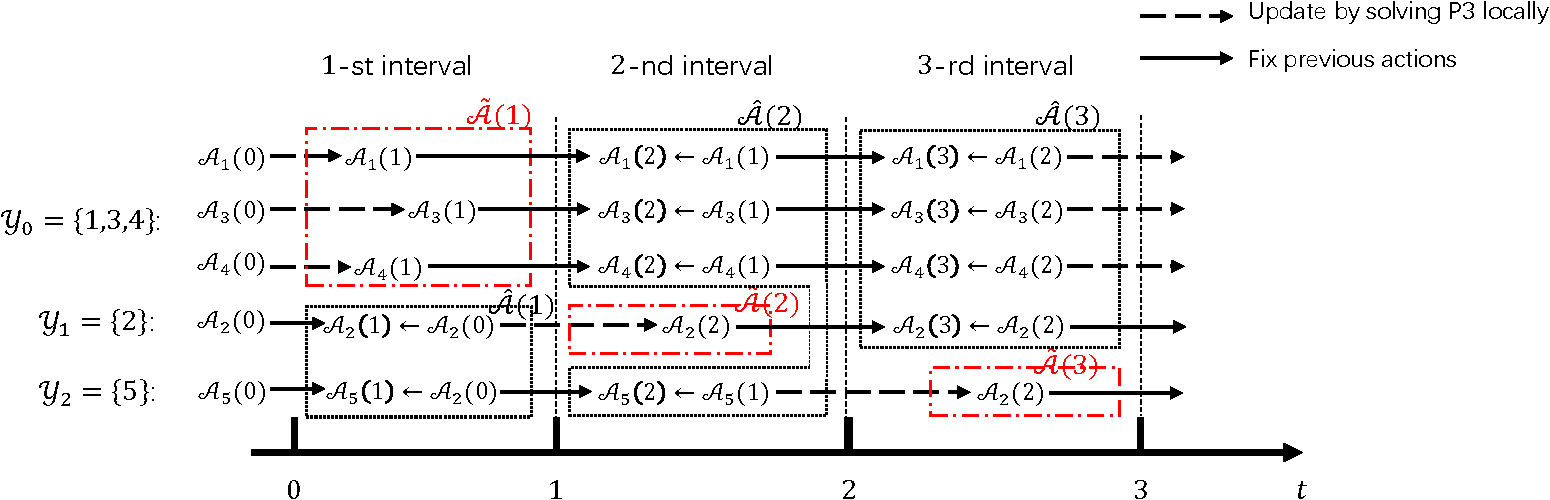
\includegraphics[width=0.60\textwidth]{update-timeline.pdf}
        \caption{The Illustration of Example \ref{exp:update}.}
        \label{fig:update_timeline}
    \end{figure*}
\end{example}

% As a remark notice that Algorithm \ref{alg_1} leads to a time-variant policy, which is referred as the proposed policy $\tilde{\Policy}$.
% At the $t$-th broadcast interval, the dispatching actions is given by
% \begin{align}
%     \tilde{\Policy}(\Stat(t), \Delay(t)) \define \tilde{\mathcal{A}}(t+1) \cup \hat{\mathcal{A}}(t+1).
% \end{align}
As a remark notice that since in Algorithm \ref{alg_1}, the computation complexity at each AP scales linearly with respect to {the size of candidate edge server set}, it can be deployed in a scenario with massive APs and edge servers, as long as the {the available number of edge servers for each AP} is limited.

\subsection{Analytical Performance Bound}
\label{subsec:analysis}
In most of the existing approximate MDP solutions \cite{mdp-bound1,mdp-bound2,mdp-bound3}, the performance is difficult to bound analytically as the approximate value function has no accurate meaning on the system cost or utility.
In the proposed algorithm, however, we derive the analytical expression for the baseline policy as the approximate.
Hence, the alternative dispatching action update can ensure to achieve a better performance than the baseline policy.
This conclusion is summarized below.
% We have the following conclusion on the performance of the above proposed algorithm.
\begin{lemma}[\hongyc{Semi-Analytical Cost Upper Bound}]
    \label{lemma:bound}
    Let $W_{\tilde{\Policy}}(\cdot)$ be the value function (average cost) of the proposed policy $\tilde{\Omega}$, i.e.,
    {\small
    \begin{align}
        W_{\tilde{\Policy}}(\Stat) \define
        \sum_{t'=1}^{\infty} \gamma^{t'-1} \mathbb{E}^{ \tilde{\Policy} } \Bracket{
            g\Paren{\Stat(t'), \tilde{\Policy}(\Stat(t'),\Delay(t'))} \Big| \Stat(1)=\Stat
        },
    \end{align}
    }
    \hongyc{(replace with a tight baseline $\tilde{\Pi}$, which is a $n$-step improved policy). }
    \hongyc{(As the the closed analytical performance improvement is hard to obtain, we develop a semi-analytical expression of the tight baseline policy $W_{\tilde{\Pi}}$, where the cost function is evaluated by integrating numerical policy improvement part and analytical evaluation fixed policy part. The semi-analytical form is elaborated as follows.)}
    {\small
    \begin{align}
        W_{\tilde{\Pi}}(\Stat(t)) = E[] + W_{?}(\Stat(t+n)),
    \end{align}
    }%
    we have
    {\small
    \begin{align}
        V(\Stat)
        \leq W_{\tilde{\Policy}}(\Stat)
        \leq W_{\Baseline}(\Stat),
        \forall \Stat.
    \end{align}
    }%
\end{lemma}
\begin{proof}
    Please refer to Appendix \ref{append_3}.
\end{proof}
Therefore, $W_{\Baseline}(\Stat)$ derived in equation (\ref{eqn:baseline}) can be used as the analytical cost upper bound of the proposed policy $\Baseline$.
Moreover, Lemma \ref{lemma:bound} also implies that the proposed policy with fixed service edge server for each AP, as long as the {static dispatching policy} is used as the baseline policy.
% the average system cost of the proposed algorithm is upper bounded by $W_{\Baseline}(\Stat)$ ($\forall \Stat$) which means it is always better than the baseline policy. 

%----------------------------------------------------------------------------------------%
\section{Reinforcement Learning Algorithm}
\label{sec:rl-alg}
\hongyc{
    In the previous section, the approximate value function $W_{\Baseline}(\Stat)$ is derived analytically.
    However, the calculation of $ W_{\Baseline}(\Stat)$ requires the priori knowledge on the distributions in this system, i.e., job arrival distributions, uploading latency distributions and computation time distributions, which are usually unknown in practice.
    Therefore, we extend the \algname~with a novel reinforcement learning approach.
    Specifically, with the explicit analytical expressions of $\tilde{W}^{\AP}_{k,m,j}$ and $\tilde{W}^{\ES}_{m,j}$ in Lemma \ref{lemma:w_ap} and Lemma \ref{lemma:w_es}, respectively, we only need to learn the following statistical parameters.
    \begin{itemize}
        \item The average arrival rate $\lambda_{k,j}$ of job arrival distribution $B_{k,j}(t)$ ($\forall k\in\apSet,j\in\jSpace$), which could be estimated directly from the job arrival events.
        \item The expectation of computation time $c_{m,j}$. Here, we further denote the observation of type-$j$ job departure from the $m$-th edge server at the $t$-th slot as $\alpha_{m,j}$ (i.e., $\alpha_{m,j}=1$ if job departures and $0$ otherwise); the computation time of the departure is denoted as $p^{c}_{m,j}(t)$ if $\alpha_{m,j}=1$; the estimation of $c_{m,j}$ is equivalent to sample a geometric distribution ($\forall m\in\esSet,j\in\jSpace$).
        \item The uploading time distribution $\mathbb{U}_{k,m,j}(\Xi)$. For convenience, we denote $\vec{u}_{k,m,j} \define [\Pr\{U_{k,m,j}\}=1, \dots, \Pr\{U_{k,m,j}\}=\Xi]$ and the estimation of $\vec{u}_{k,m,j}$ is easy by observing the uploading job state $\vec{R}^{(k)}_{m,j}(t)$ change on APs ($\forall k\in\apSet,m\in\esSet,j\in\jSpace$).
    \end{itemize}
    As a remark notice that, the observation for statistical parameters estimation is at timeslot-level and could be shared with other APs and edge servers via broadcast information. And the update of statistics would take effect exactly when the broadcast information is partially received by the conflict AP set.
    Hence, the convergence is not affected by the information staleness introduced in periodic broadcast and \brlatency.
    The reinforcement learning algorithm is given as follows.
}

\begin{algorithm}[ht]
    \caption{Reinforcement Learning Algorithm}\label{alg_3}
    \DontPrintSemicolon % Some LaTeX compilers require you to use \dontprintsemicolon instead
    \KwIn{$\vec{R}^{(k)}_{m,j}(t)$, $B_{k,j}(t)$, ${p}^{c}_{m,j}(t)$}
    \KwOut{$\hat{\lambda}_{k,j}(t)$, $\hat{c}_{m,j}(t)$, $\hat{\vec{u}}_{k,m,j}(t)$}
    Initialize $\hat{\lambda}_{k,j}(t)$, $\hat{c}_{m,j}(t)$, $\hat{\vec{u}}_{k,m,j}(t)$ as zero ($\forall k\in\apSet,m\in\esSet,j\in\jSpace$).\;
    $t \gets 0$\;
    \While{not converge}{
        $t \gets t + 1$\;
        \ForPar{$k\in\apSet$, $m\in\esSet$, $j\in\jSpace$}{
            $\hat{\lambda}_{k,j}(t) \gets \frac{t-1}{t} \hat{\lambda}_{k,j}(t-1) + \frac{1}{t} I[B_{k,j}(t)=1]$\;
            $\hat{c}_{m,j}(t) \gets \frac{t-1}{t} \hat{c}_{m,j}(t-1) + \frac{1}{t} [\alpha_{m,j}{p}^{c}_{m,j}(t) + (1-\alpha)]$\;
            $\hat{\vec{u}}_{k,m,j}(t) \gets \frac{t-1}{t} \hat{\vec{u}}_{k,m,j}(t-1) + \frac{
                I[\vec{R}^{(k)}_{m,j}(t)=0] \cdot I[\vec{R}^{(k)}_{m,j}(t-1)\neq 0]
            }{
                t || I[\vec{R}^{(k)}_{m,j}(t)=0] \cdot I[\vec{R}^{(k)}_{m,j}(t-1)\neq 0] ||_{2}
            }$\;
        }
    }
    % \For{$t=0,1,2,\dots$}{
        % \tcc{Get the index of the subset to update at $t$.}
        % \ForPar{$y \in \mathcal{Y}_{n}$}{
        % }
    % }
\end{algorithm}

\begin{theorem}[Convergence of Algorithm \ref{alg_3}]
    When $t\to\infty$, Algorithm \ref{alg_3} will converge, i.e., $\lim_{t\to\infty} \hat{\lambda}_{k,j}(t) = {\lambda}_{k,j}$, $\lim_{t\to\infty} \hat{c}_{m,j}(t) = {c}_{m,j}$ and $\lim_{t\to\infty} \hat{\vec{u}}_{m,j}(t) = \vec{u}_{m,j}$ ($\forall k\in\apSet,m\in\esSet,j\in\jSpace$).
    % As a remark notice that, the convergence of $\hat{u}_{m,j,\xi}$ could be accelerated via cooperation of APs sharing stale observation which obviously dose not affect the correctness of estimation.
\end{theorem}

\begin{proof}
    Note that the statistics $\hat{\lambda}_{k,j}$, $\hat{c}_{m,j}$ and $\hat{\vec{u}}_{m,j}$ are updated with unbiased observation, the convergence is straightforward according to Theorem 1 in Chapter I of \cite{voinov2012unbiased}.
\end{proof}

\begin{remark}[Learning Efficiency of Algorithm \ref{alg_3}]
    \hongyc{
        In conventional reinforcement learning algorithms, the value function should be evaluated for at least a large subset of system states or state-action paris before the convergence.
        Moreover, the value function of a system state can be updated only when this system state appears after state transitions (which is impractical for our problem which is with enormous state space or action space), which leads to large computation complexity and convergence time.
        In the proposed reinforcement learning algorithm, however, we only learn the unknown statistics of the value function by tracking their unbiased observations.
        Hence, the proposed algorithm could converge faster.
    }
\end{remark}
%----------------------------------------------------------------------------------------%
%----------------------------------------------------------------------------------------%